

\tikzset{every picture/.style={line width=0.75pt}} %set default line width to 0.75pt

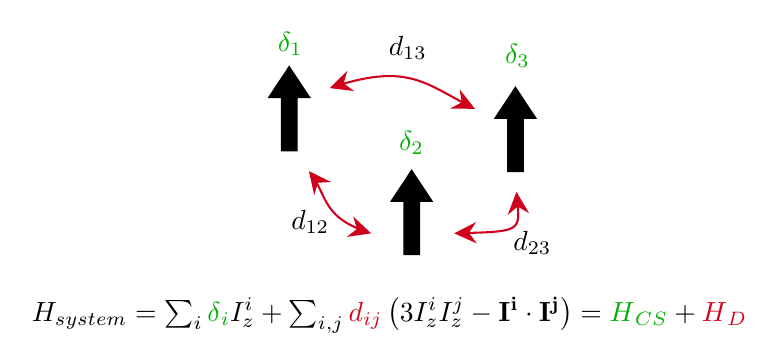
\begin{tikzpicture}[x=0.75pt,y=0.75pt,yscale=-1,xscale=1]
%uncomment if require: \path (0,321); %set diagram left start at 0, and has height of 321

%Up Arrow [id:dp3616533286619681]
\draw  [fill={rgb, 255:red, 0; green, 0; blue, 0 }  ,fill opacity=1 ] (142,55.33) -- (151.5,41) -- (161,55.33) -- (155.03,55.33) -- (155.03,81) -- (147.97,81) -- (147.97,55.33) -- cycle ;
%Up Arrow [id:dp5012912754811447]
\draw  [fill={rgb, 255:red, 0; green, 0; blue, 0 }  ,fill opacity=1 ] (201,105.33) -- (210.5,91) -- (220,105.33) -- (214.03,105.33) -- (214.03,131) -- (206.97,131) -- (206.97,105.33) -- cycle ;
%Up Arrow [id:dp52188591349806]
\draw  [fill={rgb, 255:red, 0; green, 0; blue, 0 }  ,fill opacity=1 ] (251,65.33) -- (260.5,51) -- (270,65.33) -- (264.03,65.33) -- (264.03,91) -- (256.97,91) -- (256.97,65.33) -- cycle ;
%Curve Lines [id:da4574392367290909]
\draw [color={rgb, 255:red, 208; green, 2; blue, 27 }  ,draw opacity=1 ]   (162.84,93.56) .. controls (169.95,104.28) and (168.51,113.13) .. (188.4,120.13) ;
\draw [shift={(191,121)}, rotate = 197.49] [fill={rgb, 255:red, 208; green, 2; blue, 27 }  ,fill opacity=1 ][line width=0.08]  [draw opacity=0] (10.72,-5.15) -- (0,0) -- (10.72,5.15) -- (7.12,0) -- cycle    ;
\draw [shift={(161,91)}, rotate = 51.91] [fill={rgb, 255:red, 208; green, 2; blue, 27 }  ,fill opacity=1 ][line width=0.08]  [draw opacity=0] (10.72,-5.15) -- (0,0) -- (10.72,5.15) -- (7.12,0) -- cycle    ;
%Curve Lines [id:da7885055809075856]
\draw [color={rgb, 255:red, 208; green, 2; blue, 27 }  ,draw opacity=1 ]   (234.47,120.9) .. controls (263.46,120.07) and (262.79,119.99) .. (261.27,103.96) ;
\draw [shift={(261,101)}, rotate = 445.16] [fill={rgb, 255:red, 208; green, 2; blue, 27 }  ,fill opacity=1 ][line width=0.08]  [draw opacity=0] (10.72,-5.15) -- (0,0) -- (10.72,5.15) -- (7.12,0) -- cycle    ;
\draw [shift={(231,121)}, rotate = 358.33] [fill={rgb, 255:red, 208; green, 2; blue, 27 }  ,fill opacity=1 ][line width=0.08]  [draw opacity=0] (10.72,-5.15) -- (0,0) -- (10.72,5.15) -- (7.12,0) -- cycle    ;
%Curve Lines [id:da5782733153480035]
\draw [color={rgb, 255:red, 208; green, 2; blue, 27 }  ,draw opacity=1 ]   (174.37,49.9) .. controls (208.59,39.07) and (217.43,48.94) .. (238.64,59.81) ;
\draw [shift={(241,61)}, rotate = 206.24] [fill={rgb, 255:red, 208; green, 2; blue, 27 }  ,fill opacity=1 ][line width=0.08]  [draw opacity=0] (10.72,-5.15) -- (0,0) -- (10.72,5.15) -- (7.12,0) -- cycle    ;
\draw [shift={(171,51)}, rotate = 341.27] [fill={rgb, 255:red, 208; green, 2; blue, 27 }  ,fill opacity=1 ][line width=0.08]  [draw opacity=0] (10.72,-5.15) -- (0,0) -- (10.72,5.15) -- (7.12,0) -- cycle    ;


% Text Node
\draw (26,150.4) node [anchor=north west][inner sep=0.75pt]    {$H_{\text{system}} =\sum _{i}\textcolor[rgb]{0,0.69,0}{\delta }\textcolor[rgb]{0,0.69,0}{_{i}} I^{i}_{z} +\sum _{i,j}\textcolor[rgb]{0.82,0.01,0.11}{d}\textcolor[rgb]{0.82,0.01,0.11}{_{ij}}\left( 3I^{i}_{z} I^{j}_{z} -\mathbf{I^{i}} \cdot \mathbf{I^{j}}\right) =\textcolor[rgb]{0,0.69,0}{H}\textcolor[rgb]{0,0.69,0}{_{\text{CS}}} +\textcolor[rgb]{0.82,0.01,0.11}{H}\textcolor[rgb]{0.82,0.01,0.11}{_{D}}$};
% Text Node
\draw (151,108.4) node [anchor=north west][inner sep=0.75pt]  [font=\normalsize]  {$d_{12}$};
% Text Node
\draw (258,118.4) node [anchor=north west][inner sep=0.75pt]  [font=\normalsize]  {$d_{23}$};
% Text Node
\draw (198,24.4) node [anchor=north west][inner sep=0.75pt]  [font=\normalsize]  {$d_{13}$};
% Text Node
\draw (144.5,22.4) node [anchor=north west][inner sep=0.75pt]  [color={rgb, 255:red, 0; green, 175; blue, 0 }  ,opacity=1 ]  {$\delta _{1}$};
% Text Node
\draw (203,70.4) node [anchor=north west][inner sep=0.75pt]  [color={rgb, 255:red, 0; green, 175; blue, 0 }  ,opacity=1 ]  {$\delta _{2}$};
% Text Node
\draw (254,28.4) node [anchor=north west][inner sep=0.75pt]  [color={rgb, 255:red, 0; green, 175; blue, 0 }  ,opacity=1 ]  {$\delta _{3}$};


\end{tikzpicture}
